\documentclass[tikz]{standalone}
\usepackage{tikz}
\usetikzlibrary{decorations.pathmorphing, arrows, shapes, trees, positioning, matrix, calc, backgrounds}
\begin{document}
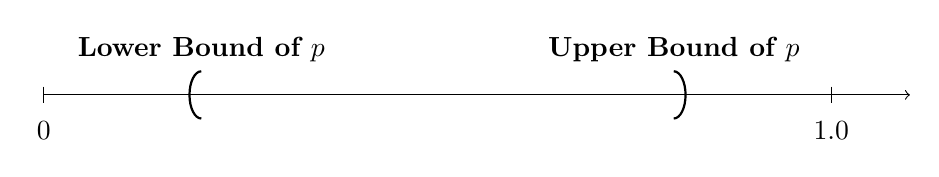
\begin{tikzpicture}
  \draw[->] (0,0) -- (11,0);
  \foreach \x in {0, 1.0} {
    \draw[shift={(\x*10,0)},color=black] (0pt,3pt) -- (0pt,-3pt);
    \draw[shift={(\x*10,0)},color=black] (0pt,-6pt) node[below] {\x};}
  \draw[thick] (2.0,-0.3) arc (270:90:0.15cm and 0.3cm);
  \node[above] at (2.0,0.3) {\textbf{Lower Bound of $p$}};
  \draw[thick] (8.0,-0.3) arc (-90:90:0.15cm and 0.3cm);
  \node[above] at (8.0,0.3) {\textbf{Upper Bound of $p$}};
\end{tikzpicture}
\end{document}